
\documentclass[letterpaper,11pt]{article}

\usepackage{latexsym}
\usepackage{amsmath}
\usepackage{amssymb}
\usepackage{unicode-math}
\usepackage{fancyhdr}
\usepackage[margin=1.0in, left=0.5in, right=0.5in, top=1.25in, headsep=10mm, headheight=15mm]{geometry}
\usepackage{graphicx}

\setmainfont{Latin Modern Roman}
\setmathfont{Latin Modern Math}

\pagestyle{fancy}
\rhead{Mech 222 Mathematics Worksheets\\ Lectures 2, 3}


\newcommand*\limitset[1]{{#1}^\prime}
% Not working in unicode math with xelatex for some reason...
% \newcommand*\closure[1]{\overline #1}
\newcommand*\closureunion[1]{{#1}\cup \limitset{#1}}
\newcommand*\interior[1]{{#1}^\circ}

% Sets of points
% The set of points within some distance #1 from #2
\newcommand*\neighbor[2]{N_{#1}({#2})}
% The neighborhood without #2
\newcommand*\delneighbor[2]{N_{#1}^*({#2})}
\newcommand*\set[1]{\{ #1 \} }
\newcommand*\conjugate[1]{\overline{#1}}
\newcommand*\sequence[2]{\set{#1}_{#2=1}^\infty}
\newcommand*\series[2]{\sum_{#2=1}^\infty #1_{#2}}
\newcommand*\compose[2]{#1 \circ #2}
\newcommand*\udisk{\mathbb{D}}
\newcommand*\disk[2]{D_{#1}(#2)}
\newcommand*\punctdisk[2]{\disk_{ #1 } - \set{#2}}
\newcommand*\complex{\mathbb{C}}
\newcommand*\naturals{\mathbb{N}}
\newcommand{\integers}{\mathbb{Z}}
\newcommand*\rationals{\mathbb{Q}}
\newcommand*\reals{\mathbb{R}}

% Function spaces
\newcommand*\cnfunc[2]{C^{#2}\left(#1 \right)}
\newcommand*\cnfuncdom[1]{C^{#1}\left(\domain \right)}
\newcommand*\linffunc[1]{L^{\infty}\left(#1 \right)}
\newcommand*\linffuncdom{L^{\infty}\left(\domain \right)}
\newcommand*\lnfunc[2]{L^{#2}\left(#1 \right)}
\newcommand*\lnfuncdom[1]{L^{#1}\left(\domain \right)}
\newcommand*\sobolev[3]{W^{#2, #3}\left(#1 \right)}
\newcommand*\sobolevdom[2]{W^{#1, #2}\left(\domain \right)}
\newcommand*\sobolevh[2]{H^{#2}\left(#1 \right)}
\newcommand*\sobolevhdom[1]{H^{#1}\left(\domain \right)}
\newcommand*\sobolevcs[3]{W_0^{#2, #3}\left(#1 \right)}
\newcommand*\sobolevcsdom[2]{W_0^{#1, #2}\left(\domain \right)}
\newcommand*\sobolevhcs[2]{H_0^{#2}\left(#1 \right)}
\newcommand*\sobolevhcsdom[1]{H_0^{#1}\left(\domain \right)}

\newcommand*\grad{D}
\newcommand*\graddir[1]{D_{#1}}
\newcommand*\lapl{∆}
\newcommand*\diffquot[1]{D^{#1}}
\newcommand*\diffquotdir[2]{D_{#2}^{#1}}

\newcommand*\domain{U}
\newcommand*\bndry[1]{\partial #1}
\newcommand*\bndrydom{\partial \domain}
\newcommand*\compactcont{\subset \subset} % U \compactcont V \rightarrow U \subset \closure{U} \subset V, where U, V are (open) domains

\newcommand*\ballunit{B_1}
\newcommand*\ball[2]{B_{#2}(#1)}
\newcommand*\bunitsurfarea[1]{\omega_{#1}}
\newcommand*\bunitsurfareadef{\omega_n}
\newcommand*\bunitvolume[1]{\alpha_{#1}}
\newcommand*\bunitvolumedef{\alpha_n}

\newcommand*\limitto[2]{\lim \limits_{#1 \rightarrow #2}}

\newcommand{\dd}[1]{\;\mathrm{d}#1}
\newcommand{\dx}{\dd{x}}
\newcommand{\dy}{\dd{y}}
\newcommand{\dz}{\dd{z}}
\newcommand{\dr}{\dd{r}}
\newcommand{\ds}{\dd{s}}
\newcommand{\dS}{\dd{S}}
\newcommand{\dt}{\dd{t}}
\newcommand*\pderiv[2]{\frac{\partial #1}{\partial #2}}
\newcommand*\nthpderiv[3]{\frac{\partial^{#3} #1}{\partial #2^{#3}}}
\newcommand*\deriv[2]{\frac{\dd{#1}}{\dd{#2}}}
\newcommand*\nthderiv[3]{\frac{\dd{^{#3} #1}}{\dd{#2^{#3}}}}

% Norms
\newcommand*\linfnorm[2]{\left\lVert#1\right\rVert_{L^{\infty}(#2)}}
\newcommand*\linfnormdom[1]{\left\lVert#1\right\rVert_{L^{\infty}(\domain)}}

\newcommand*\lnorm[3]{\left\lVert#1\right\rVert_{L^{#2}(#3)}}
\newcommand*\lnormdom[2]{\left\lVert#1\right\rVert_{L^{#2}(\domain)}}

\newcommand*\hnorm[3]{\left\lVert#1\right\rVert_{H^{#2}(#3)}}
\newcommand*\hnormdom[2]{\left\lVert#1\right\rVert_{H^{#2}(\domain)}}

\newcommand*\wnorm[4]{\left\lVert#1\right\rVert_{W^{#2, #3}(#4)}}
\newcommand*\wnormdom[3]{\left\lVert#1\right\rVert_{W^{#2, #3}(\domain)}}

\DeclareMathOperator{\res}{res}
\DeclareMathOperator{\sign}{sign}
\DeclareMathOperator{\diam}{diam}
\DeclareMathOperator{\partition}{Partition}

% Matrix computations
\newcommand*\trace[1]{\text{tr}\left( #1 \right)}

% Average integral from https://tex.stackexchange.com/questions/759/average-integral-symbol
\def\Xint#1{\mathchoice
{\XXint\displaystyle\textstyle{#1}}%
{\XXint\textstyle\scriptstyle{#1}}%
{\XXint\scriptstyle\scriptscriptstyle{#1}}%
{\XXint\scriptscriptstyle\scriptscriptstyle{#1}}%
\!\int}
\def\XXint#1#2#3{{\setbox0=\hbox{$#1{#2#3}{\int}$ }
\vcenter{\hbox{$#2#3$ }}\kern-.6\wd0}}
\def\ddashint{\Xint=}
\def\dashint{\Xint-}
\def\avgint{\dashint}


\begin{document}
\section*{Integration in polar coordinates}
Recall that polar coordinates are defined as follows:
\begin{align*}
  x = r \cos(\theta), & \hspace{5mm} y = r \sin(\theta)\\
  r = \sqrt{x^2 + y^2}, & \hspace{5mm} \theta = \arctan \left( \frac{y}{x} \right)
\end{align*}
To write an integral in polar form, we need three things:
\begin{enumerate}
  \item A function of polar coordinates, $\hat{f}(r, \theta)$
  \item Boundaries for the polar coordinates
  \item A differential area element
\end{enumerate}
For 1, given $f(x, y)$, we can compute $\hat{f}(r, \theta)$ as $f(r \cos(\theta), r \sin(\theta))$\\
For 2, we need constraints for $r$, $\theta$, generally by drawing a picture and inspecting the geometry; ie, choose either r or thete as the outer integral, find the maximum and minimum values of it, then find the maximum and minimum values for the inner integral when holding the outer integral variable constant.
Recall that these coordinates are periodic in $\theta$, so the boundaries on $\theta$ may only be implied.\\
For 3, consider small area produced by slightly increasing $r$ and $\theta$:
\begin{figure}[h]
  \centering 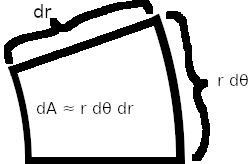
\includegraphics[width=100px]{mech222/worksheet_1b_polar_diff_elem.png}
  \caption{Polar coordinates differential area element}
\end{figure}
This isn't a rigorous justification, but provides an intuitive explanation.
However, this leaves out the detail that the order matters for this!
Fubini's theorem lets us swap the order of $\dd{\theta}$ and $\dr$, but it doesn't take the additional $r$ term with it.
That is:
$$
\int \int \hat{f}(r, \theta) \dd{A} = \int \int \hat{f}(r, \theta) r \dd{\theta} \dr = \int \int \hat{f}(r, \theta) r \dr \dd{\theta} \neq \int \int \hat{f}(r, \theta) \dr \, r \dd{\theta}
$$
The $r$ term must be included in the integral over the radial coordinate.

\subsection*{Example}
Integrate $f(x, y) = x^2 + 2 x y + y^2$ over the torus (donut) with inner radius of $1$ and outer radius of $2$.

\begin{enumerate}
  \item $\hat{f}(r, \theta) = f(r \cos(\theta), r \sin(\theta)) = r^2 ( 1 + 2 \cos(\theta) \sin(\theta) ) = r^2 (1 + \sin(2 \theta))$
  \item There are no constraints on $\theta$ over the torus; so we arbitrarily choose $\theta_{min} = 0$ and $\theta_{max} = 2 \pi$ as this covers the entire domain exactly once.
    $r$ ranges from $1$ to $2$ independently of $\theta$.
  \item Our integral is then $\int \limits_{1}^{2} \int \limits_{0}^{2 \pi} r^2 (1 + \sin(2 \theta)) r \dd{\theta} \dr$
\end{enumerate}
\begin{align*}
  & \int \limits_{1}^{2} \int \limits_{0}^{2 \pi} r^2 (1 + \sin(2 \theta)) r \dd{\theta} \dr
    = \int \limits_{1}^{2} \int \limits_{0}^{2 \pi} r^3 (1 + \sin(2 \theta)) \dd{\theta} \dr
    = \int \limits_{1}^{2} 2 \pi r^3 \dr
    = \frac{1}{2} \pi r^4 \bigg \rvert_{1}^{2}
    = \frac{1}{2} \pi (16 - 1)
\end{align*}
Compare this to computing the integral in Cartesian coordinates, which requires 4 separate integrals.

\subsection*{Problems}
First, draw the regions to be integrated over.
Clearly label the boundaries and their equations for one of the polar variables (ie, for a cardiod, the boundary equation is $r = 2 (1 - \cos(\theta))$).
Use polar coordinates to compute the following integrals.
\begin{enumerate}
  \item $f(x, y) = 1$, $D = \set{(r, \theta) | 0 \leq r < 5, 0 < \theta < 2 \pi}$ is the radius $5$ ball\\
    \newline
    \newline
    \newline
    \newline
    \newline
  \item $f(x, y) = 5 x^6 + 15 x^4 y^2 + 15 x^2 y^4 + 5 y^4$, $D = \set{(r, \theta) | 0 \leq r < 1, 0 < \theta < 2 \pi}$ is the unit ball.
    \newline
    \newline
    \newline
    \newline
    \newline
  \item $\hat{f}(r, \theta) = \frac{\sin(\theta)}{r}$, $D$ is the torus with inner radius 1 and outer radius 2.
    \newline
    \newline
    \newline
    \newline
    \newline
  \item $f(x, y) = \frac{x}{x^2 + y^2}$, $D$ is the cardiod defined by $r = 1 - \cos(\theta)$.
    \newline
    \newline
    \newline
    \newline
    \newline
  \item $f(x, y) = \frac{y^2}{x}$, $D$ is the right triangle with vertices $(0, 0)$, $(1, 0)$, $(1, 1)$.
    \newline
    \newline
    \newline
    \newline
    \newline
  \item $f(x, y) = e^{x^2} \frac{x}{\sqrt{x^2 + y^2}}$,
    $D$ is the wedge between the unit circle and the rays from the origin at $\theta = 0$ and $\theta = \frac{2}{3} \pi$.
    \newline
    \newline
    \newline
    \newline
    \newline
\end{enumerate}
\end{document}
